\let\negmedspace\undefined
\let\negthickspace\undefined
\documentclass[journal]{IEEEtran}
\usepackage[a5paper, margin=10mm, onecolumn]{geometry}
%\usepackage{lmodern} % Ensure lmodern is loaded for pdflatex
\usepackage{tfrupee} % Include tfrupee package

\setlength{\headheight}{1cm} % Set the height of the header box
\setlength{\headsep}{0mm}     % Set the distance between the header box and the top of the text
\usepackage{gvv-book}
\usepackage{gvv}
\usepackage{cite}
\usepackage{amsmath,amssymb,amsfonts,amsthm}
\usepackage{algorithmic}
\usepackage{graphicx}
\usepackage{textcomp}
\usepackage{xcolor}
\usepackage{txfonts}
\usepackage{listings}
\usepackage{enumitem}
\usepackage{mathtools}
\usepackage{gensymb}
\usepackage{comment}
\usepackage[breaklinks=true]{hyperref}
\usepackage{tkz-euclide} 
\usepackage{listings}
% \usepackage{gvv}                                        
\def\inputGnumericTable{}                                 
\usepackage[latin1]{inputenc}                                
\usepackage{color}                                            
\usepackage{array}                                            
\usepackage{longtable}                                       
\usepackage{calc}                                             
\usepackage{multirow}                                         
\usepackage{hhline}                                           
\usepackage{ifthen}                                           
\usepackage{lscape}
\begin{document}

\bibliographystyle{IEEEtran}
\vspace{3cm}

\title{9.3.12B}
\author{EE24BTECH11027 - satwikagv}
% \maketitle
% \newpage
% \bigskip
{\let\newpage\relax\maketitle}

\renewcommand{\thefigure}{\theenumi}
\renewcommand{\thetable}{\theenumi}
\setlength{\intextsep}{10pt} % Space between text and floats


\numberwithin{equation}{enumi}
\numberwithin{figure}{enumi}
\renewcommand{\thetable}{\theenumi}
\textbf{Question}:\\
Plot the solution of the differential equation: 
\begin{align}
    y^{\prime\prime} +xy^\prime + xy = x. 
\end{align}
\textbf{Solution}:\\
\textbf{RK4 method}:\\
Let assume
\begin{align}
    y^\prime=z
\end{align}
substituting the eq \brak{0.2} in eq  \brak{0.1} we get,
\begin{align}
    z'+xz+xy=x\\
    z'=x\brak{1-y-z}
\end{align}
Let 
\begin{align}
    z'=f\brak{x,y,z}\\
    f\brak{x,y,z}=x\brak{1-y-z}
\end{align}
To update $y$ and $z$ first we need to find the intermediate slopes of $y$ and $z$ those are given by
\begin{align}
    k_{1,y}=h\brak{z_n}\\
	k_{2,y}=h\brak{z_n+\frac{k_{1,z}}{2}}\\
    k_{3,y}=h\brak{z_n+\frac{k_{2,z}}{2}}\\
    k_{4,y}=h\brak{z_n+k_{3,z}}\\
    k_{1,z}=hf\brak{x_n,y_n,z_n}\\
    k_{2,z}=hf\brak{x_n+\frac{h}{2},y_n+\frac{k_{1,y}}{2},z_n+\frac{k_{1,z}}{2}}\\
    k_{3,z}=hf\brak{x_n+\frac{h}{2},y_n+\frac{k_{2,y}}{2},z_n+\frac{k_{2,z}}{2}}\\
    k_{4,z}=hf\brak{x_n+h,y_n+k_{3,y},z_n+k_{3,z}}
\end{align} 
The next values of $x$, $y$ and $z$ are given by
\begin{align}
	x_{n+1}=x_n+h\\
    y_{n+1}= y_n + \frac{1}{6}\brak{k_{1,y}+2k_{2,y}+2k_{3,y}+k_{4,y}}\\
    z_{n+1}= z_n + \frac{1}{6}\brak{k_{1,z}+2k_{2,z}+2k_{3,z}+k_{4,z}}
\end{align}
On iterationg the eqs from \brak{0.7} to \brak{0.17} over 100 times we get some values of $y$.\\
Here we assume the initial conditions as
\begin{align}
    x_0=0\\y_0=0\\z_0=1\\h=0.1
\end{align}
By plotting the values of $y$ we get in eq \brak{0.16} we get the graph of the solution of the given differential equation\\
\textbf{Method of Differences}\\
To plot the curve of the given differential equation $\brak{0.1}$ we can do it using the method of finite differences which is a numerical technique for solving complex differential equations by approximating derivatives with differences.\\
The approximated forward derivative of $y\brak{x}$ is given as:\\
\begin{align}
    y^\prime_n\approx\frac{y_{n+1}-y_n}{h}
\end{align}
On rearranging we get,
\begin{align}
    y_{n+1}=y_n+y^\prime_n\brak{h}
\end{align}
And also 
\begin{align}
    x_{n+1}=x_n+h
\end{align}
The approximated forward derivative of second order of $y\brak{x}$ is given as:\\
\begin{align}
    y^{\prime\prime}_n\approx \frac{y^\prime_{n+1}-y^\prime_n}{h}
\end{align}
Substitute eq $\brak{0.22}$ in eq $\brak{0.25}$ we get,
\begin{align}
    y^{\prime\prime}_n\approx\frac{y_{n+2}-2y_{n+1}+y_n}{h^2}
\end{align}
Substitute  eq $\brak{0.22}$ and eq $\brak{0.26}$ in eq $\brak{0.1}$ and on rearanging we get,
\begin{align}
    y_{n+2}=y_{n+1}\brak{2-hx_n} +y_n\brak{-1+hx_n-h^2x_n}+h^2x_n
\end{align}
We need to assume two initial conditions as it is a second order differential equation. \\So here we assume the initial conditions as 
\begin{align}
    x_0=0\\y_0=0\\y^\prime_0=1\\h=0.1
\end{align}
substitute eq $\brak{0.28}$, eq $\brak{0.29}$ and eq $\brak{0.30}$ in eq $\brak{0.1}$\\ we get 
\begin{align}
    y^{\prime\prime}\brak{0}=0
\end{align}
Substitute eq $\brak{0.29}$ and eq $\brak{0.30}$ in eq $\brak{0.23}$
\begin{align}
    y_1=y_0+y^\prime_0(0.1)\\
    y_1=0.1
\end{align}
For the rest of the points use eq $\brak{0.27}$ we get the other points.\\
The graph sim1 represents the graph obtained by the method of finite differences\\
The graph sim2 represents the graph obtained by the RK4 method
\begin{figure}[h!]
   \centering
   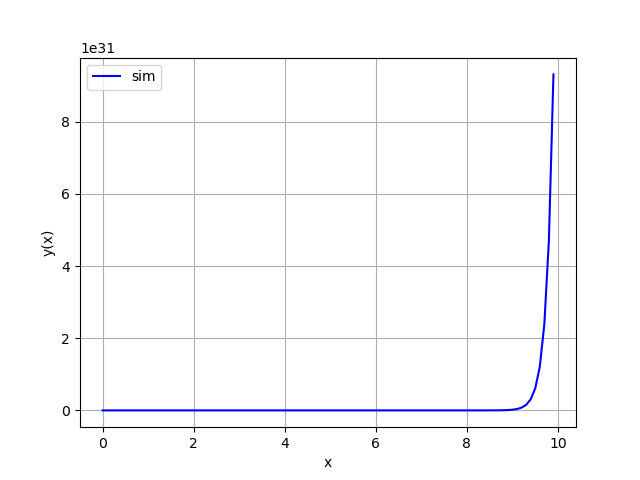
\includegraphics[width=\columnwidth]{figs/fig.png}
\end{figure}
\end{document}
